

\begin{frame}[fragile]{The central and local repository}
  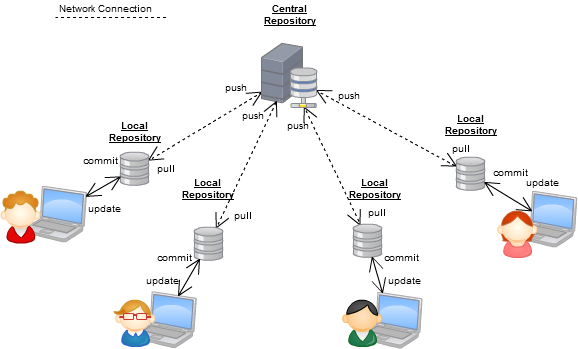
\includegraphics[height=0.9\textheight, width=\textwidth]{images/distributed}
\end{frame}



\begin{frame}[fragile]{Configuration}
Before starting to use git, you may want to configure it as follows:

	\begin{lstlisting}
$ git config --global user.name "First Last"
$ git config --global user.email "email@example.com"
$ git config --global color.diff "auto"
$ git config --global color.status "auto"
$ git config --global color.branch "auto"
	\end{lstlisting}
\end{frame}

\begin{frame}[fragile]{Create/Clone a repository}
	\begin{lstlisting}
$ # Clone a remote repository
$ git clone https://github.com/C3BI-pasteur-fr/tutorials.git |\pause|

$ # or create a local repository in the current folder
$ git init
	\end{lstlisting}
\end{frame}




%\begin{frame}[fragile]{Add a new file on the remote repository}
%\begin{lstlisting}
%$ # create your file
%$ touch README.rst
%
%$ Check the status of your repo
%$ git status
%
%$ # add it to your local repository
%$ git add README.rst
%
%$ Check the status 
%$ git status
%
%$ # commit to your local repository
%$ git commit README.rst -m "Meaningful message"
%
%$ Check the status 
%$ git status
%
%$ # Send to the server for everybody
%$ git push 
%
%$ Check the status 
%$ git status
%\end{lstlisting}
%\end{frame}

%\begin{frame}
%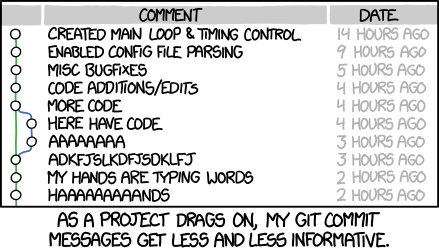
\includegraphics[height=0.9\textheight, width=\textwidth]{images/git_commit}
%\end{frame}


\section{Working together: branching}

\begin{frame}
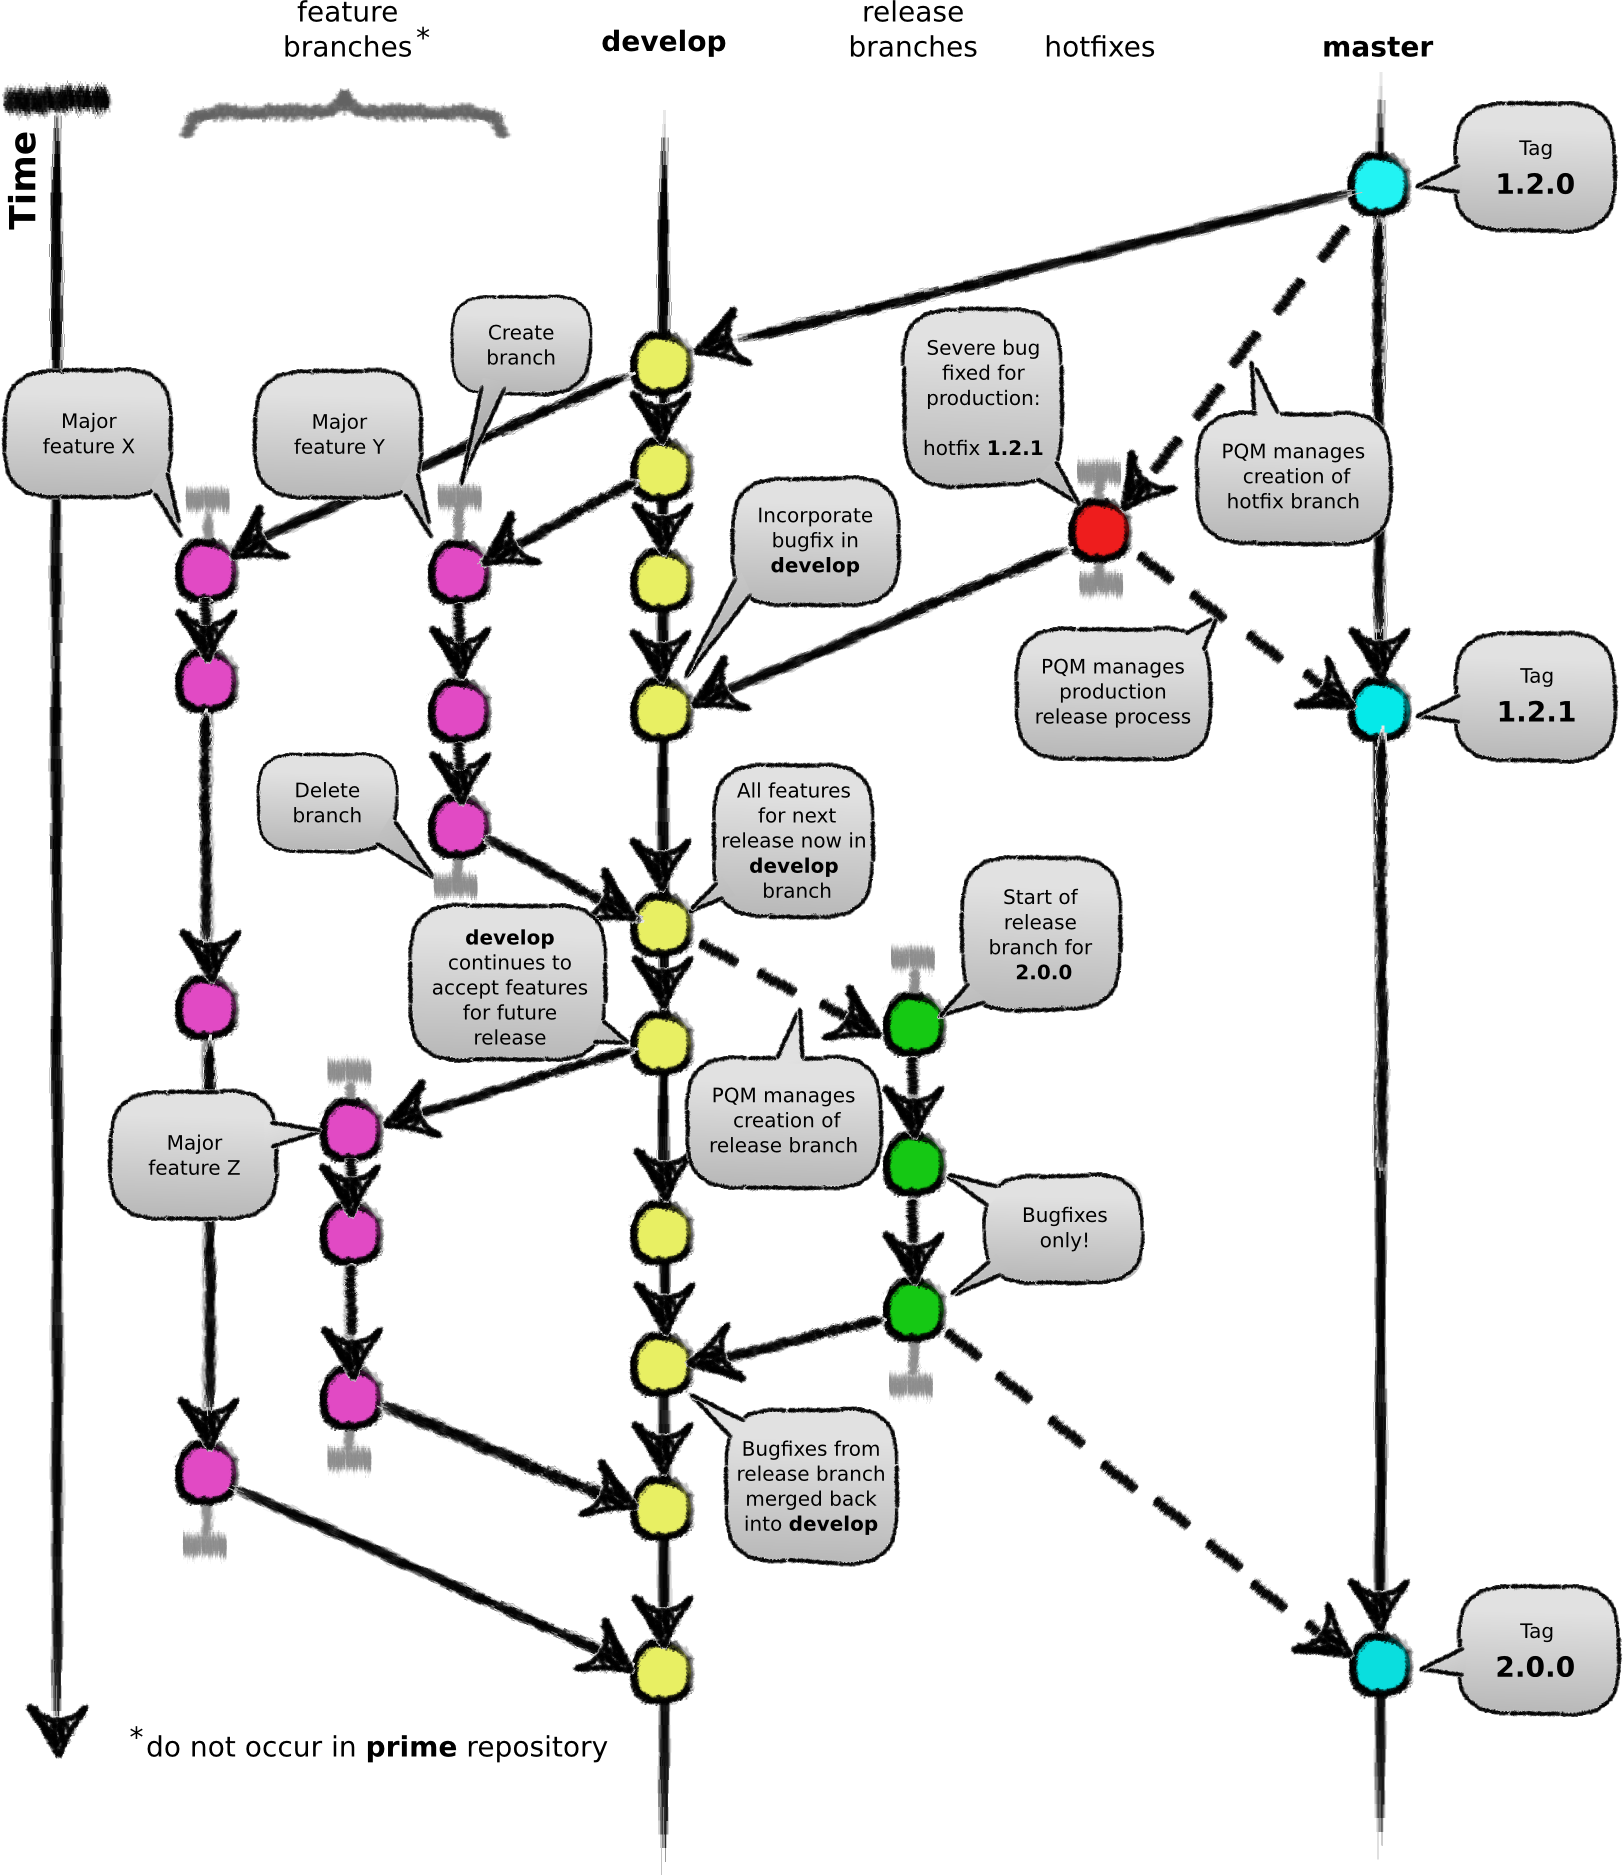
\includegraphics[height=0.9\textheight, width=\textwidth]{images/gitflow}
\end{frame}

\begin{frame}[fragile]{Write a new feature/bug fix}
	\begin{enumerate}
		\item Create a new branch
		\item Implement a new feature/Fix a bug
		\begin{enumerate}
			\item Step 1 towards new feature/bug fix
			\item Commit
			\item Step 2 towards new feature/bug fix
			\item Commit
			\item \ldots
		\end{enumerate}
		\item Update the master
		\item Delete this branch 
	\end{enumerate}
\end{frame}

\begin{frame}[fragile]{Step 1. Create a new branch locally}
	\begin{lstlisting}
$ # Which branches do we have?
$ git branch -a |\pause|
* master
remotes/origin/HEAD -> origin/master
remotes/origin/master
remotes/origin/services |\pause|

$ # Create a branch for our feature/bug fix...
$ git branch feature
$ # ... and switch to this branch
$ git checkout feature 
Switched to a new branch "feature" |\pause|

$ # or create + switch in one command
$ git checkout -b feature 
Switched to a new branch "feature"
  	\end{lstlisting}
\end{frame}

\begin{frame}[fragile]{Step 2. Implement a new feature/Fix a bug}
  	\begin{lstlisting}
$ # Add files to index (to-be-committed)
$ git add main.py __init__.py |\pause|

$ # Remove files from index
$ git reset HEAD __init__.py |\pause|

$ # Look at current index state
$ git status
On branch feature
Changes to be committed:
  (use "git reset HEAD <file>..." to unstage)

	modified:   main.py

Changes not staged for commit:
  (use "git add <file>..." to update what will be committed)
  (use "git checkout -- <file>..." to discard changes in working directory)

	modified:   __init__.py |\pause|

$ # Commit (in our local repository!)
$ git commit -m "Fixed TSS positions on - strand"
[feature fd07832] Fixed TSS positions on - strand
 1 file changed, 1 insertion(+)
  	\end{lstlisting}
\end{frame}


\begin{frame}[fragile]{Step 3. Update the master}
  	\begin{lstlisting}
# Switch to master
$ git checkout master
Switched to branch 'master' |\pause|


$ # Reapply our commits on the master branch
$ git rebase feature
First, rewinding head to replay your work on top of it...
Fast-forwarded master to feature.
	\end{lstlisting}
\end{frame}

\begin{frame}[fragile]{Step 4. Remove the branch}
  	\begin{lstlisting}
$ # Remove local branch
$ git branch -d feature
Deleted branch feature (was fd86490). |\pause|
	\end{lstlisting}
\end{frame}


\begin{frame}[fragile]{The scenario we've just seen}
    \begin{columns}
\begin{column}{0.6\textwidth}
\small
	\begin{enumerate}
		\item Created a new branch \textbf{locally}
		\item Implemented a new feature/bug fix
		\begin{enumerate}
			\item Step 1 towards new feature
			\item Commit
			\item Step 2 towards bug fix
			\item Commit
			\item \ldots
		\end{enumerate}
		\item \textbf{Reapplied} the commits from this branch on the master \textbf{locally}
		\item Deleted this branch \textbf{locally} (it never existed elsewhere)
		
		\item Push changes to the remote server (origin)
		\begin{lstlisting}
		$ git push origin master
		\end{lstlisting}
	\end{enumerate}
\end{column}
\begin{column}{0.9\textwidth}
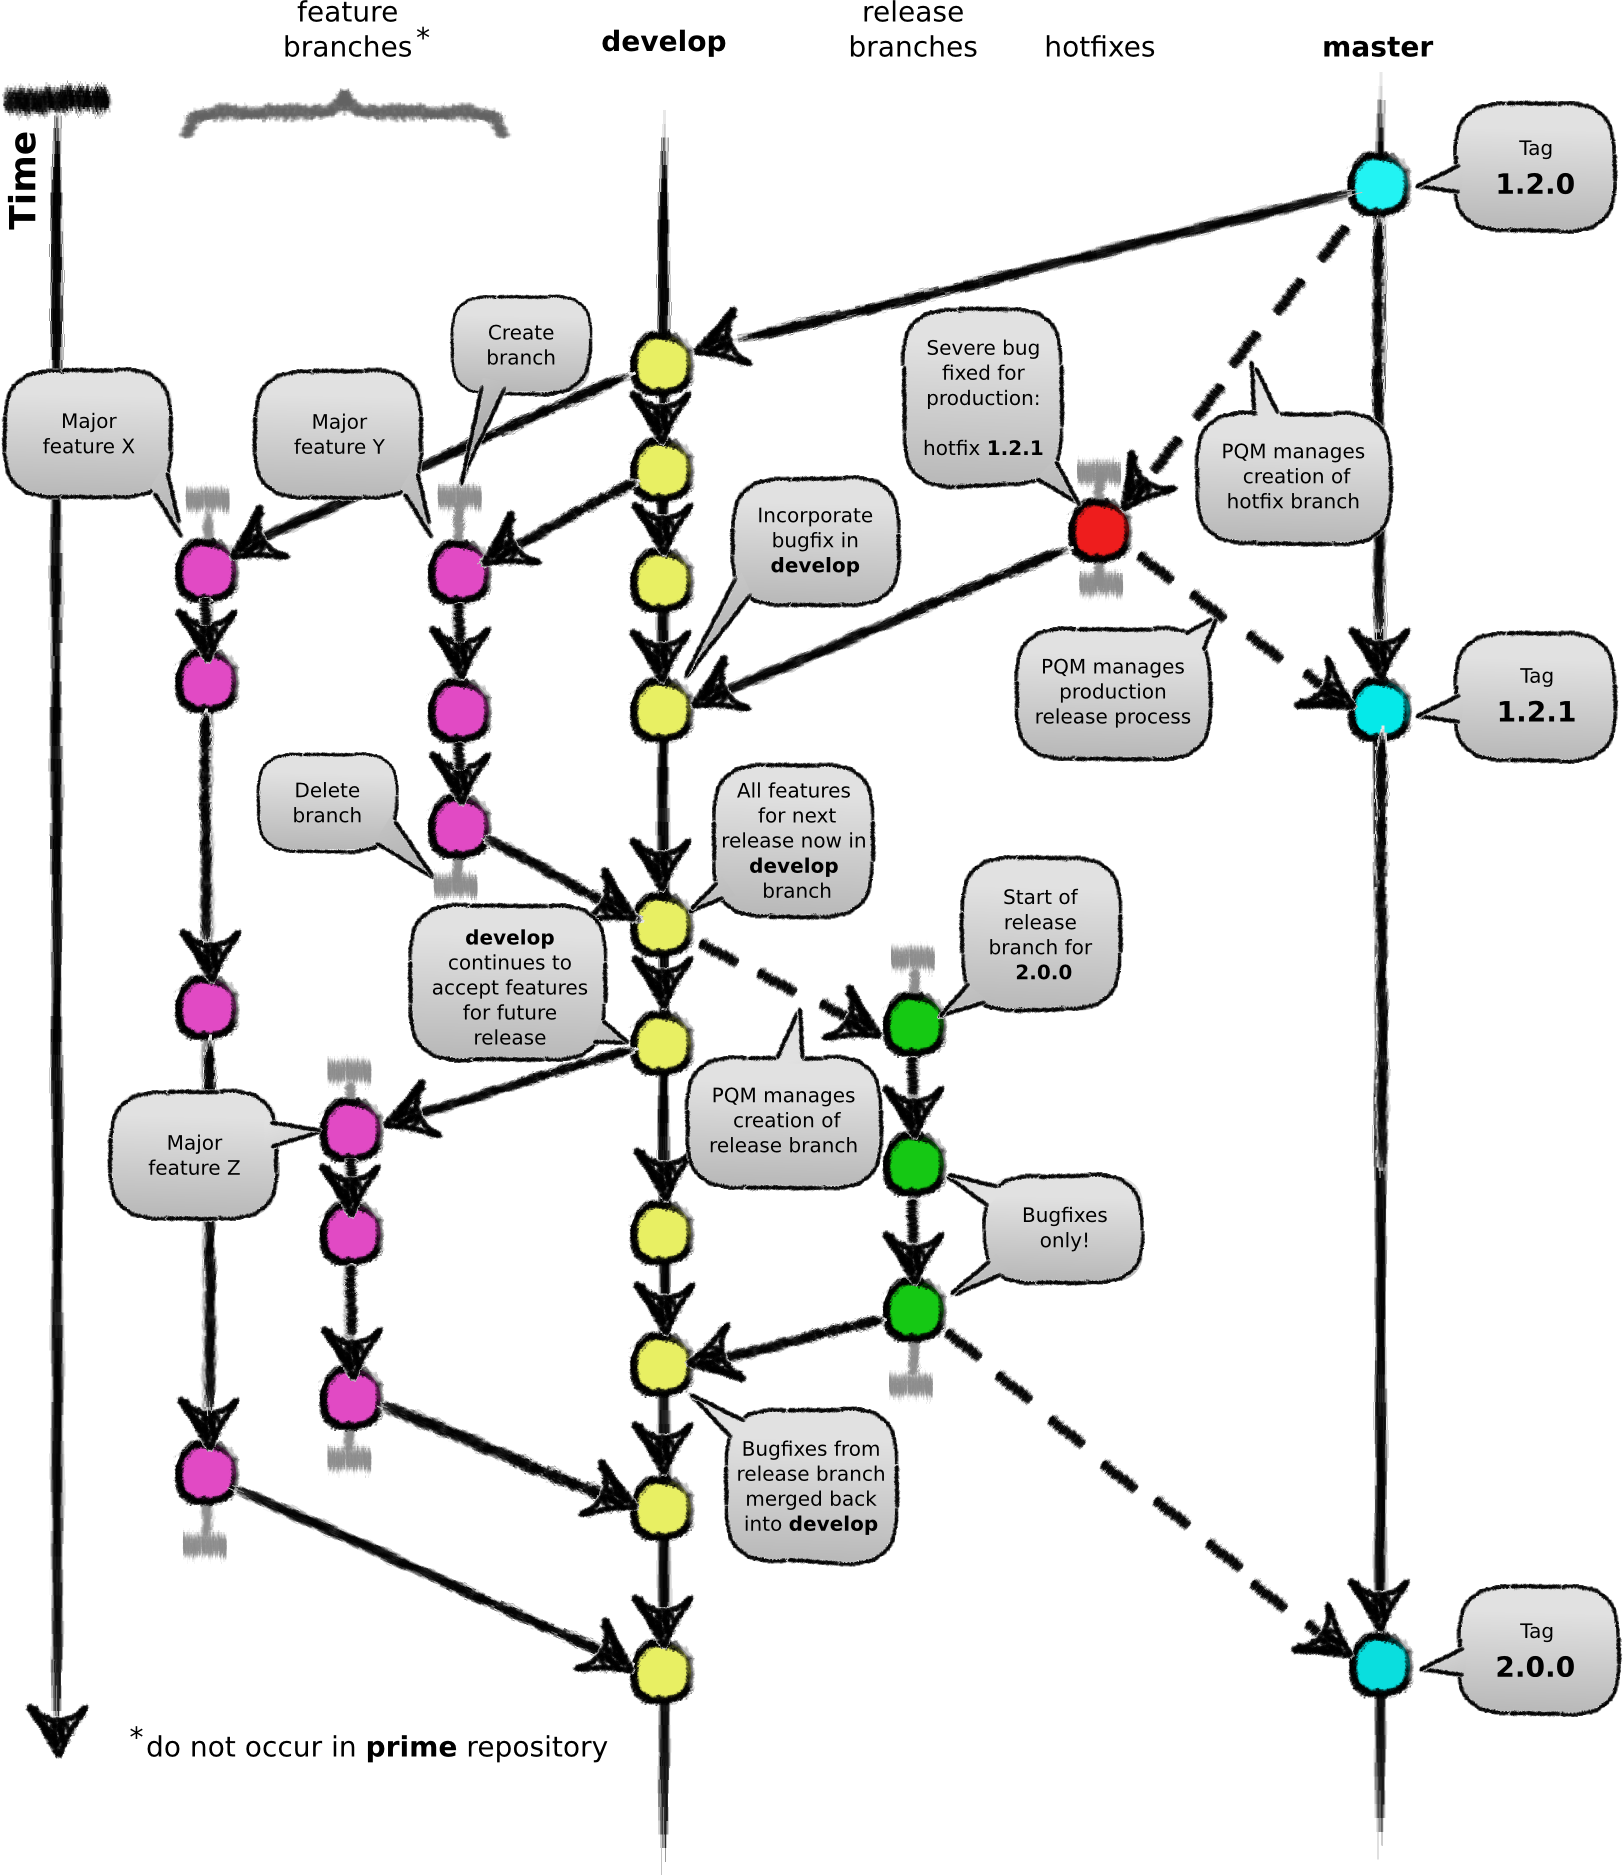
\includegraphics[height=0.7\textheight, width=0.6\textwidth]{images/gitflow}
\end{column}
\end{columns}

	\pause
	\textit{What if I am not the only one working on this feature/bug?}
\end{frame}

\begin{frame}[fragile]{Publishing the branch on origin}
	\begin{lstlisting}
$ # Push our branch 'feature' to a new branch 'feature' (will be created) on origin
$ git push origin feature:feature |\pause|

$ # From now on, to push (committed) changes we can...
$ git push origin feature |\pause|
	\end{lstlisting}
\end{frame}

\begin{frame}[fragile]{Getting updates from origin}
	\begin{lstlisting}
$ # Pull updates from origin
$ git pull |\pause|
     ...
There is no tracking information for the current branch.
Please specify which branch you want to merge with.
See git-pull(1) for details.

    git pull <remote> <branch> |\pause|
    
$ # Pull (what?) branch feature (from where?) from origin
$ git pull origin feature |\pause|

$ # We can also update config...
$ # (from where?)
$ git config branch.feature.remote origin
$ # (what?)
$ git config branch.feature.merge feature

$ # ...so that from now on, we can pull just by...
$ git pull
	\end{lstlisting}
\end{frame}


\begin{frame}[fragile]{Joining someone else's branch}
	\begin{lstlisting}
$ git checkout --track -b bug origin/bug
Branch bug set up to track remote branch refs/remotes/origin/bug.
Switched to a new branch "bug"
	\end{lstlisting}
	
	\pause
	\begin{tiny}
	{\color{eclipsePurple} Beware:} \textit{pull origin bug} would have merged the changes from the remote branch \textit{bug} into our current local branch!
\end{tiny}
\end{frame}

\begin{frame}[fragile]{Update the master}
  	\begin{lstlisting}
$ # Switch to master
$ git checkout master
Switched to branch "master" |\pause|

$ # Merge
$ git merge feature |\pause|


$ # Note that if the feature only existed locally, 
$ # we could have used rebase instead of merge:
$ git rebase feature |\pause|


$ # Do not forget to push
$ git push
	\end{lstlisting}
\end{frame}


\begin{frame}[fragile]{Remove the branch}
  	\begin{lstlisting}
$ # Remove local branch feature
$ git branch -d feature
Deleted branch feature (was fd86490). |\pause|


$ # Remove remote branch feature
$ git push origin :feature
- [deleted] feature
	\end{lstlisting}
\end{frame}


\begin{frame}[fragile]{The scenario we've just seen}
	\begin{enumerate}
		\item Created a new branch locally \textbf{and published it on the remote origin}
		\item Implemented a new feature/Fixed a bug
		\begin{enumerate}
			\item Step 1 towards new feature/bug fix
			\item Commit \textbf{(and maybe push to origin)}
			\item \ldots
			\item \textbf{Pull other developers' changes from origin}
			\item \ldots
		\end{enumerate}
		\item \textbf{Merged} this branch with the master \textbf{locally}
		\item \textbf{Pushed changes to origin}
		\item Deleted this branch locally \textbf{and on origin}
	\end{enumerate}
	\pause
	\textit{What if I want to work in several branches in parallel?}
\end{frame}

\begin{frame}[fragile]{Working in several branches in parallel}
	\begin{tiny}
		\begin{lstlisting}
$ # On branch A: did some changes, but not yet ready to commit...
$ # Want to switch to branch B. |\pause| Checkout?
$ git checkout master
error: Your local changes to the following files would be overwritten by checkout:
	main/basic_git.tex
Please, commit your changes or stash them before you can switch branches.
Aborting |\pause|

$ # Save the changes first.
$ git stash
Saved working directory and index state WIP on basic_git: 30fb6e8 Fixed typos
HEAD is now at 30fb6e8 Fixed typos |\pause|

$ # Now we can switch to another branch and work there...
$ git checkout master
Switched to branch 'master'
$ ...
		\end{lstlisting}
	\end{tiny}
\end{frame}

\begin{frame}[fragile]{Working in several branches in parallel}
	\begin{tiny}
		\begin{lstlisting}
$ # Back on branch A: How do I get my changes back?
$ # Which stashes are there?
$ git stash list
stash@{0}: WIP on master: ceef0bd Merge pull request #1 from C3BI-pasteur-fr/services
stash@{1}: WIP on basic_git: 30fb6e8 Fixed typos |\pause|

$ # Apply the stash
$ git stash apply stash@{1}
On branch basic_git
Changes not staged for commit:
  (use "git add <file>..." to update what will be committed)
  (use "git checkout -- <file>..." to discard changes in working directory)

	modified:   basic_git.tex
	... |\pause|
	
$ # Remove this stash from stash list
$ git stash drop stash@{1}
Dropped stash@{1} (739c015cafdc37e22a45d97868c3d03bc940eadf)
		\end{lstlisting}
	\end{tiny}
\end{frame}

\begin{frame}{Summary}
	\begin{tiny}
    \begin{itemize}
        \item[] {\color{eclipseBlue}git init} -- create an empty repository
        \item[] {\color{eclipseBlue}git clone <repository>} -- clone a repository into a new directory
        \item[]
        \item[] {\color{eclipseBlue}git branch -a} -- list existing branches
        \item[] {\color{eclipseBlue}git branch <branch>} -- create a branch
        \item[] {\color{eclipseBlue}git checkout <branch>} -- switch to the branch 
        \item[]
        \item[] {\color{eclipseBlue}git status} -- show the working tree status
        \item[] {\color{eclipseBlue}git add <filepath>} -- add a file to the index (to be committed)
        \item[] {\color{eclipseBlue}git commit -m <message>} -- record changes to the local repository
        \item[]
        \item[] {\color{eclipseBlue}git pull <from where?> <which branch?>} -- fetch and integrate changes
        \item[] {\color{eclipseBlue}git push <where?> <to which branch?>} -- push the changes the remote repository
        \item[]
        \item[] {\color{eclipseBlue}git merge <branch>} -- merge the selected branch into the current branch
        \item[] {\color{eclipseBlue}git rebase <branch>} -- reapply commits from the branch on top of the current branch
        \item[]
        \item[] {\color{eclipseBlue}git stash} -- record the current state of the working directory and the index, and clean the working directory
        \item[] {\color{eclipseBlue}git stash list} -- list the stashes that currently exist
        \item[] {\color{eclipseBlue}git stash apply <stash>} -- return to the state recorded in this stash
        \item[]
        \item[] {\color{eclipseBlue}git log [-{}-graph]} -- see commit logs
        \item[]
        \item[] {\color{eclipseBlue}git config [-{}-global] <key> <value>} -- set config option
    \end{itemize}
    
    \begin{center}
    	Detailed docs: \url{https://git-scm.com/docs}
    \end{center}
    \end{tiny}
\end{frame}
